\setcounter{page}{1}


\section{Introducción}
El enrutamiento dinámico es un proceso mediante el cual los routers intercambian información de enrutamiento y actualizan sus tablas de manera automática. Este enfoque permite que los routers se adapten dinámicamente a los cambios en la red, como la adición o eliminación de enlaces, asegurando la selección de las rutas más eficientes para el envío de paquetes de datos. Los protocolos de enrutamiento dinámico, como EIGRP, OSPF y RIP, facilitan el intercambio de información entre routers y el cálculo de las mejores rutas.

El protocolo EIGRP (Enhanced Interior Gateway Routing Protocol) es un protocolo avanzado de enrutamiento híbrido, desarrollado por Cisco, que combina las mejores características de los protocolos de vector de distancia y estado de enlace. EIGRP utiliza métricas como el ancho de banda, la carga, la latencia y la fiabilidad para determinar las rutas más óptimas para los paquetes de datos. Gracias a su eficiencia y escalabilidad, EIGRP es ampliamente utilizado en redes de tamaño mediano y grande (\cite{cisco}).

En esta práctica, se llevará a cabo la configuración del enrutamiento dinámico utilizando el protocolo EIGRP. El objetivo principal es profundizar en el funcionamiento e implementación de este protocolo. Para ello, se configurarán los routers y se establecerán rutas dinámicas empleando EIGRP. Además, se implementará un servidor web para realizar pruebas de conectividad, y se ajustarán los anchos de banda de las interfaces de los routers. Esta práctica permitirá comprender a fondo el funcionamiento del enrutamiento dinámico y su aplicación en redes de computadoras.
\section{Objetivos}
    \begin{itemize}
        \item Realizar enrutamiento dinámico con base en el protocolo EIGRP.
        \item Calcular el costo del enrutamiento de acuerdo a la trayectoria indicada por la tabla de enrutamiento.
    \end{itemize}

\section{Desarrollo del Trabajo}
    \subsection{Topología de red}
        Para el Desarrollo de la práctica se ha planteado la siguiente topología de red, la cual se muestra en la Figura~\ref{fig:topologia} y se compone de tres routers y tres servidores. Los routers están conectados entre sí mediante enlaces seriales, y los servidores están conectado a un diferente router. La topología de red se ha diseñado de manera que los routers puedan intercambiar información de enrutamiento y establecer rutas dinámicas utilizando el protocolo EIGRP.
    \begin{figure}[H]
        \centering
        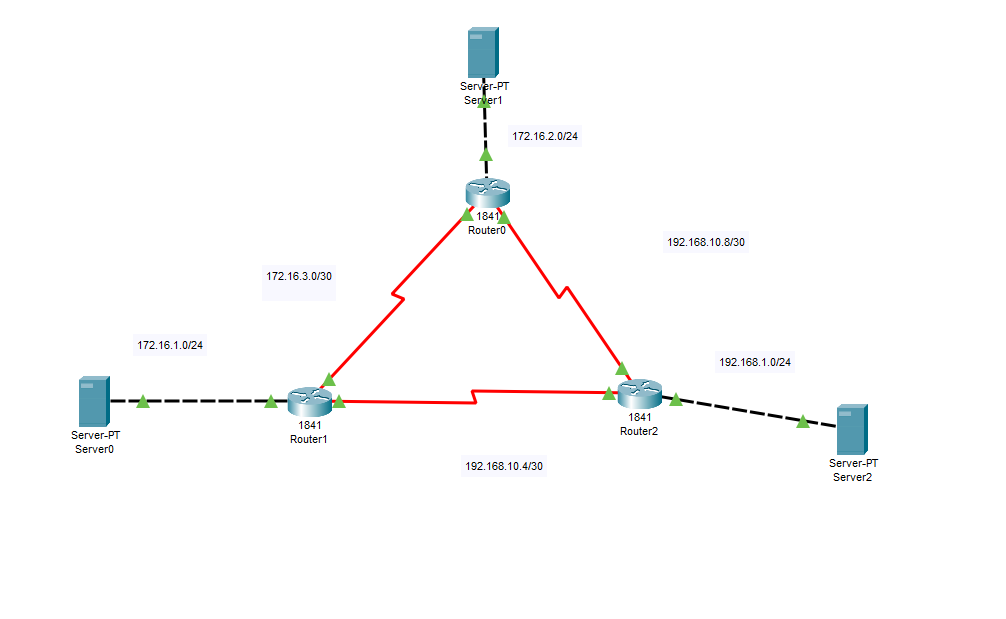
\includegraphics[width=0.8\textwidth]{img/Topologia.png}
        \caption{Topología de red}
        \label{fig:topologia}
    \end{figure}

    Para que todos los routers funcionen correctamente, nuestros compañeros deben tener la misma topología de red. Además, es necesario colaborar con los compañeros que tienen los otros routers para asegurarse de que la configuración de los dispositivos se realice de manera adecuada. Para esta práctica, utilizaremos el router 3, que fue asignado por el profesor.
    
    \subsection{Calculo de las wildcard}
    Para las wildcard necesarias a nuestro router asignado, realizaremos una tabla en la que se puede observar la dirección, la máscara y la wildcard de cada una de las direcciones de red asignadas. A continuación, se muestra la tabla con los cálculos realizados.
        \begin{table}[H]
            \centering
            \begin{tabular}{c|c|c}
                \textbf{Dirección} & \textbf{Máscara} & \textbf{Wildcard} \\
                \hline
                192.168.10.8 & 255.255.255.252 & 0.0.0.3 \\
                192.168.10.4 & 255.255.255.252 & 0.0.0.3  \\
                192.168.1.0 & 255.255.255.0 & 0.0.0.255 \\
            \end{tabular}
            \caption{Ejemplo de tabla con dirección IP, máscara, wildcard y dirección de red.}
        \end{table}
        Para obtener nuestra wildcard, utilizaremos la fórmula indicada por el profesor, en la cual restamos la máscara de subred de la dirección de broadcast de la siguiente manera:

        \begin{equation}
            \textbf{Wildcard} = \texttt{255.255.255.255} - \texttt{255.255.255.252}
           \end{equation}
        
        Esta ecuación nos dará como resultado la wildcard necesaria para configurar nuestro router en las redes conectadas a él, las cuales requieren dicha configuración.
    \subsection{Configuración del Servidor}
    Para la configuración del servidor, inicialmente crearemos un mensaje en HTML para que, al conectarse a la dirección IP del servidor, se muestre un mensaje de bienvenida. A continuación, se presenta el código HTML que se utilizará para la configuración del servidor.
        \begin{figure}[H]
            \centering
            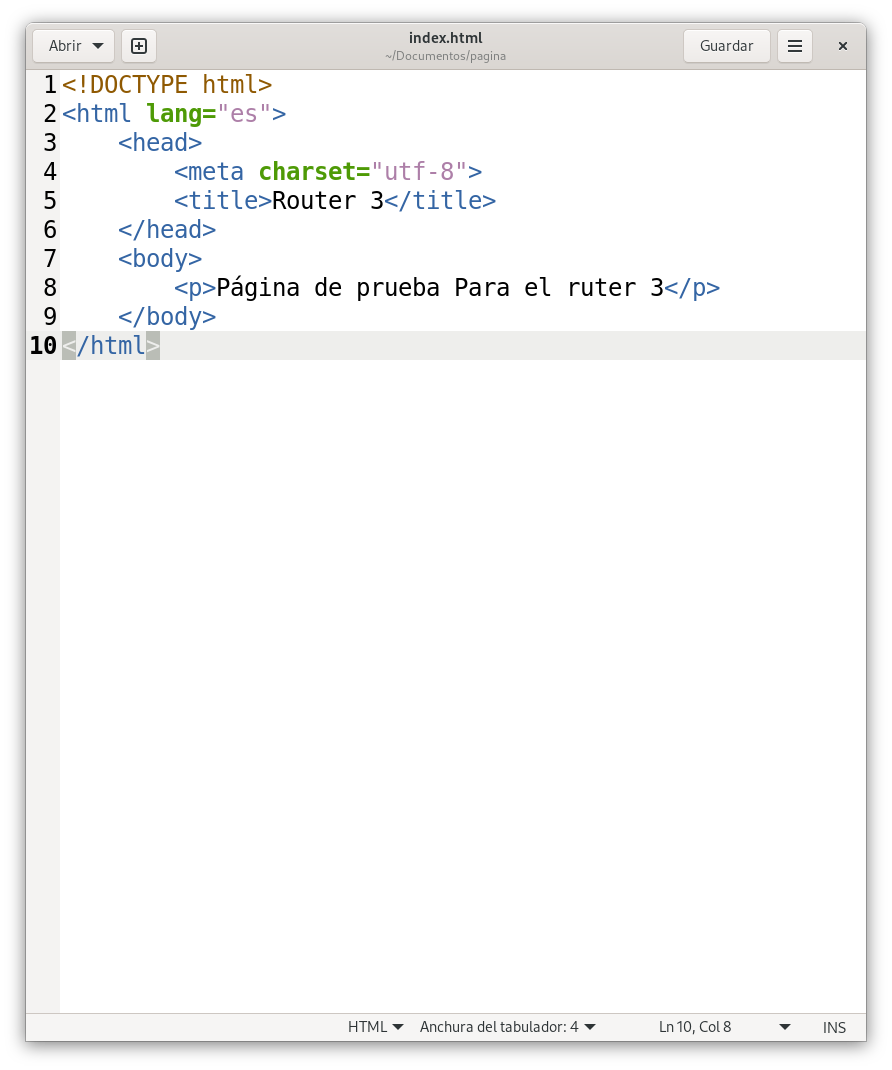
\includegraphics[width=0.5\textwidth]{img/codigo.png}
            \caption{Configuración del mensaje del servidor}
            \label{fig:serverCodigo}
        \end{figure}
        En la imagen anterior se puede observar el código HTML que se utilizará para la configuración del servidor. Este código se guardará en un archivo con la extensión .html. Al momento de encender el servidor, cualquier dispositivo que ingrese a la IP del servidor debería ver el mensaje configurado en el código HTML.

    \subsection{Configuración del router}
        Para la configuración del router, se debe realizar la configuración de las interfaces del router, la configuración de los protocolos de enrutamiento y la configuración de las rutas dinámicas. A continuación, se muestra la configuración de las Ip's del router.

        En la siguiente imagen podremos observar la configuración de las Ip's de los distintos puertos del router 3.
        \begin{figure}[H]
            \centering
            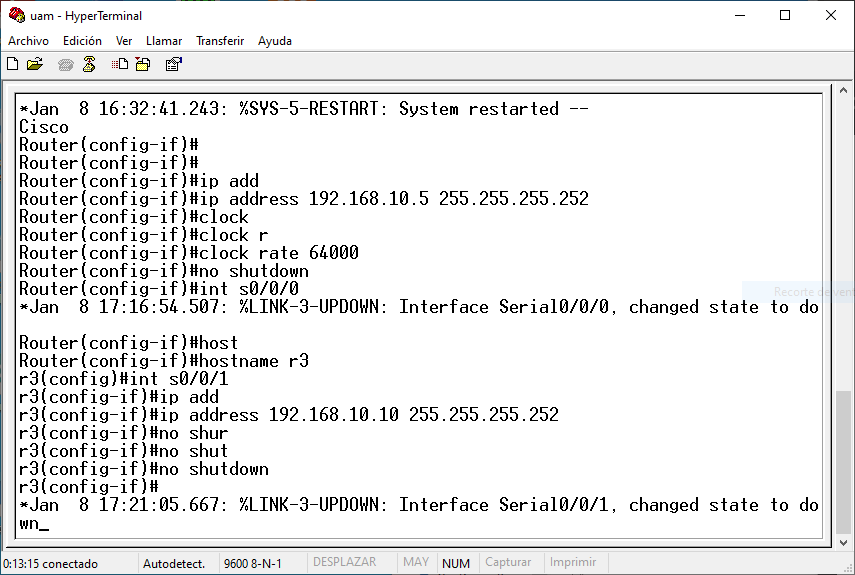
\includegraphics[width=0.6\textwidth]{img/routerip.png}
            \caption{Configuración de las ip's de los routers}
            \label{fig:router}
        \end{figure}
        En esta imagen se puede apreciar la configuración de las direcciones IP que conectan el Router 1 con el Router 2, así como la configuración del DTE (Data Terminal Equipment) para la interfaz serial 0/0/1 en el Router 1 y para la interfaz serial 0/0/0 en el Router 2. Además, se configuran otros parámetros relacionados con las interfaces de ambos routers.

    \subsection{Configuración del protocolo}

    Para esta práctica, en todos los routers de la clase utilizaremos el protocolo EIGRP (Enhanced Interior Gateway Routing Protocol) para el enrutamiento dinámico. EIGRP es un protocolo de enrutamiento avanzado de tipo híbrido, desarrollado por Cisco, que combina las mejores características de los protocolos de enrutamiento de vector de distancia y estado de enlace. El objetivo es profundizar en el funcionamiento del enrutamiento dinámico y su implementación. A continuación, se presenta la configuración de los routers para implementar el protocolo EIGRP.

    \begin{figure}[H]
        \centering
        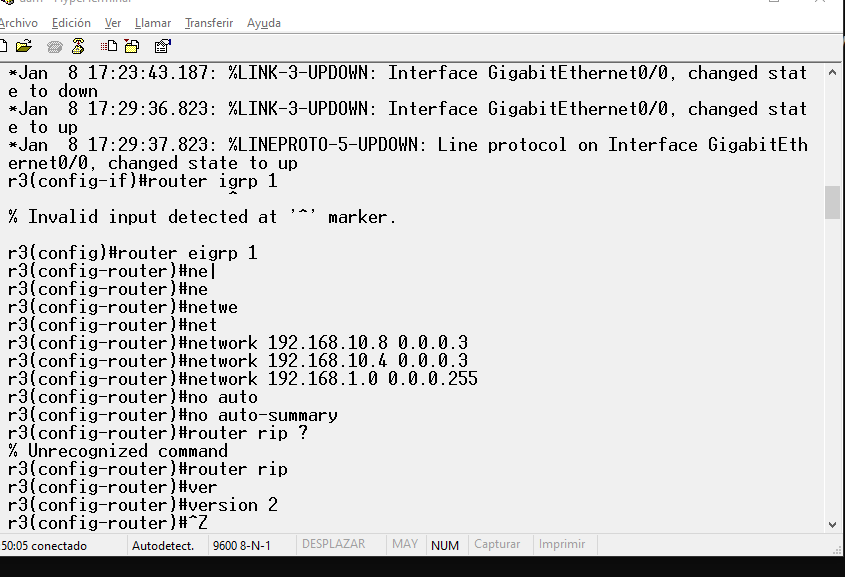
\includegraphics[width=0.6\textwidth]{img/eigrp.png}
        \caption{Configuración del protocolo EIGRP}
        \label{fig:eigrp}
    \end{figure}

    En esta imagen se puede observar cómo se configura el protocolo EIGRP en los routers, en este caso, se muestra la configuración del Router 3. En la configuración, se puede apreciar el número de AS (Autonomous System) que se utilizará; en este caso, se emplea el número 1. Además, se configura la red que se utilizará para el enrutamiento dinámico.

    También se puede observar que, al ingresar las redes según el protocolo EIGRP, es necesario especificar las redes de las interfaces que se van a configurar. En este caso, se configuran las redes que el router puede visualizar. Para esta práctica, las redes configuradas son \textbf{192.168.10.8}, \textbf{192.168.10.4} y \textbf{192.168.1.0}, con sus correspondientes máscaras wildcard.
    
    \subsection{configuración de los anchos de banda}
    Para la configuración de los anchos de banda, se debe ajustar el ancho de banda de las interfaces de los routers. A continuación, se muestra la configuración de los anchos de banda de las interfaces de los routers.
    En este caso, la práctica requiere configurar un ancho de banda de 1024 Kbps para la red \textbf{192.168.10.10}, tal como se muestra en la siguiente imagen:
    \begin{figure}[H]
        \centering
        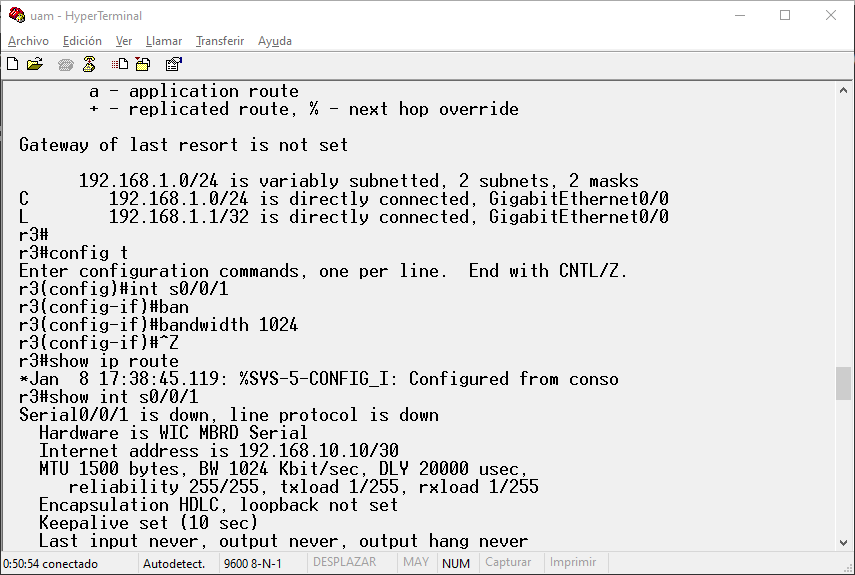
\includegraphics[width=0.6\textwidth]{img/bandwidth.png}
        \caption{Configuración del ancho de banda}
        \label{fig:bandwidth}
    \end{figure}
    En la imagen anterior, se puede observar la configuración del ancho de banda de la interfaz serial 0/0/0 del Router 3. En la configuración, se especifica el ancho de banda de la interfaz, que en este caso es de 1024 Kbps. Este ancho de banda se configura para la red.

    \subsection{Pruebas del servidor}
    Para probar el servidor, se debe ingresar a la dirección IP del servidor en un navegador web. Al ingresar a la dirección IP del servidor, se debería mostrar el mensaje de bienvenida configurado en el servidor. A continuación, se muestra la prueba del servidor.

    \begin{figure}[H]
        \centering
        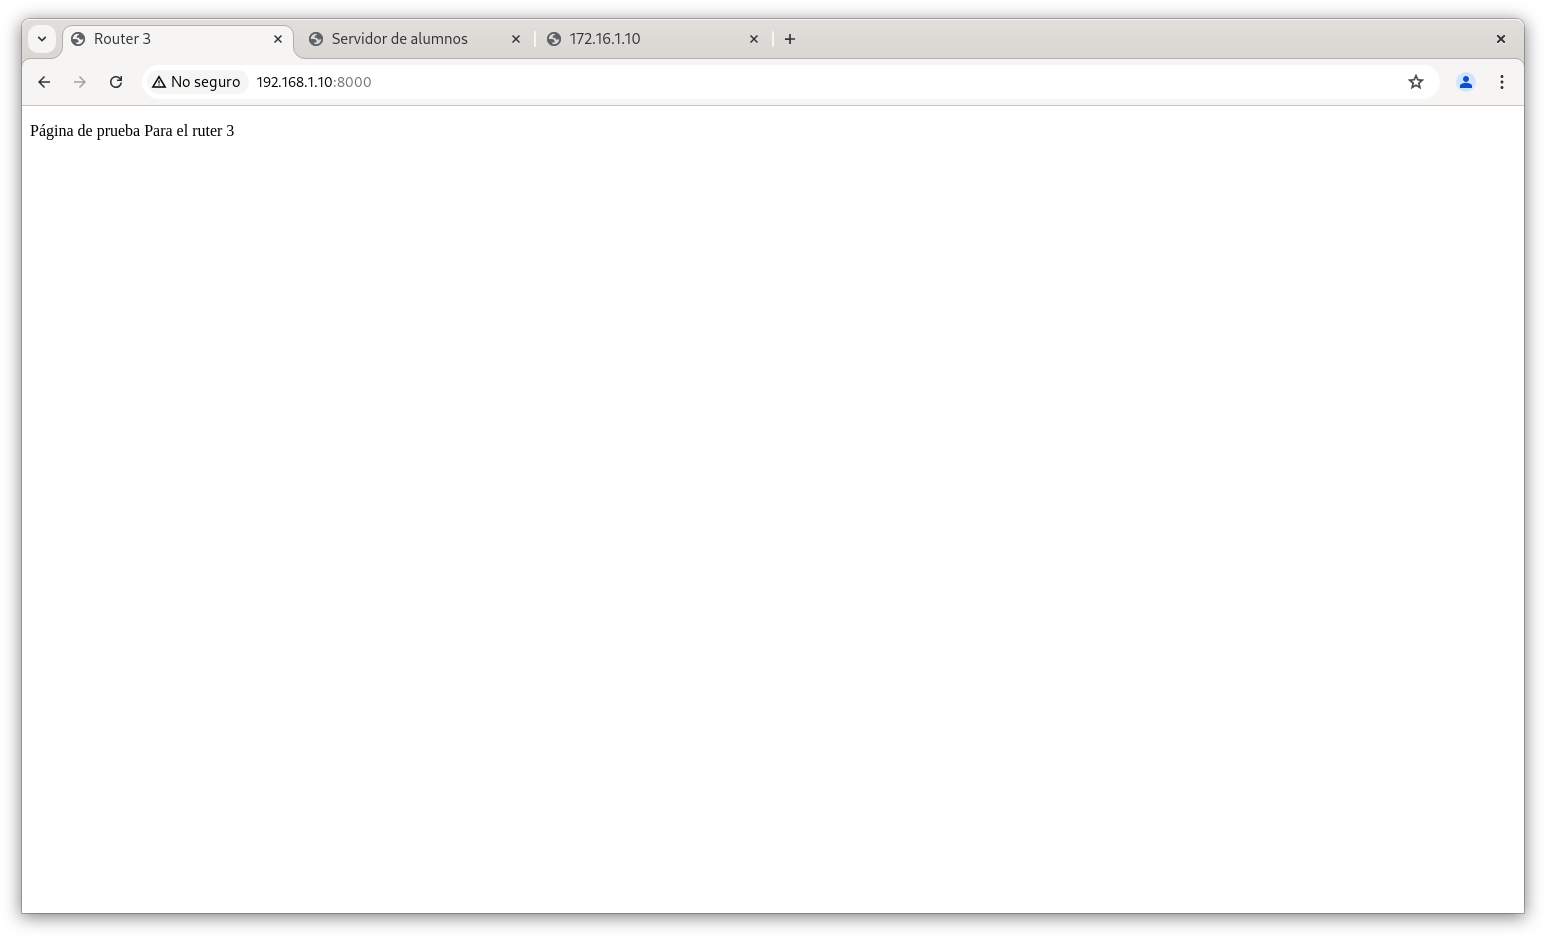
\includegraphics[width=0.6\textwidth]{img/prueba.png}
        \caption{Prueba del servidor}
        \label{fig:prueba}
    \end{figure}
    En la imagen anterior, se puede observar la prueba del servidor. Al ingresar a la dirección IP del servidor en un navegador web, se muestra el mensaje de bienvenida configurado en el servidor. Esto indica que el servidor está funcionando correctamente y que la configuración se realizó de manera adecuada.


\section{Conclusiones}
    \begin{itemize}
        \item Diego Alexis Moreno Valero - 2243900185 \\
        La práctica demostró la implementación exitosa del enrutamiento dinámico con el protocolo EIGRP, configurando routers, servidores y anchos de banda de forma eficiente. Se verificó la conectividad mediante pruebas funcionales, destacando la colaboración en redes complejas y las ventajas del protocolo en términos de eficiencia. Aunque se cumplieron los objetivos, es recomendable incluir análisis más profundos y métricas para validar los resultados. En general, el ejercicio consolidó conocimientos clave en diseño y administración de redes.
        \item Luis Ángel Cruz Díaz - 2183038433 \\
        La práctica permitió comprender el funcionamiento del enrutamiento dinámico y su implementación en redes de computadoras. Se logró configurar los routers y establecer las rutas dinámicas mediante el protocolo EIGRP. Además, se configuró un servidor web para realizar pruebas de conectividad y se ajustaron los anchos de banda de las interfaces de los routers. La práctica permitió profundizar en el enrutamiento dinámico y su implementación, así como en el cálculo del costo del enrutamiento de acuerdo a la trayectoria indicada por la tabla de enrutamiento.
    \end{itemize}


% --- Para agregar un apéndice
%\newpage
%\appendix
%\appendixpage
%\addappheadtotoc
%\section{Nombre del apéndice}